% !TeX root = ../main.tex
\section{Background}

\add{This section introduces the
elements on which the rest of the report relies. We first present IO500,
the benchmark used to measure the performance of HPC storage systems,
together with its structure, its scoring rules, and the parameters that
can be tuned. We then describe IOPS, the framework used to automate the
benchmark executions and to explore the parameter space. The section ends
with Bayesian Optimization, the search method investigated in this work.} 


\subsection{IO500}

IO500 is a benchmark suite designed to evaluate the I/O performance of
storage systems used in High Performance Computing (HPC). It was created
to provide a common and reproducible way of measuring storage performance
across different systems and configurations~\cite{io500about}.

Rather than measuring a single aspect of I/O performance, IO500 combines
several benchmarks that represent different types of storage operations.
The results can then be used both to characterise a system and to compare
it with other systems through the public IO500 ranking~\cite{io500list}.

In this work, IO500 is used as the objective to optimise. The following
subsections describe how the suite is organised, which benchmarks it uses,
how its score is computed, and which execution rules and configuration
parameters are relevant to the experiments.

\subsubsection{Benchmark structure}

IO500 is a benchmark suite rather than a single benchmark program. It
combines several benchmarks that evaluate different aspects of I/O
performance. The suite provides a common framework for running these
benchmarks and collecting their results under the same experimental
conditions~\cite{io500about}.

The benchmark is organised into a sequence of tests. Each test runs a
specific benchmark on the storage system and produces a performance
measurement. These measurements are kept separately because they
represent different aspects of I/O performance. For example, a benchmark
may focus on the amount of data transferred per second, while another
may measure the rate of file-system metadata operations.

The benchmarks are executed using a set of parameters that describe how
the benchmark should use the available computing and storage resources.
These parameters can include the number of compute nodes, the number of
processes, and file-system settings. The same benchmark can therefore
produce different results depending on the configuration used for the
run.

After the individual benchmarks have been executed, their results are
combined to produce the overall IO500 score. The score provides a single
value that can be used to compare different storage systems or different
configurations of the same system. The individual results are also
important because they make it possible to identify which aspects of I/O
performance contribute to the final score.

IO500 also defines common rules for submitting results to the public
ranking. A submission contains not only the measured performance but also
information about the system and the configuration used during the
experiment~\cite{io500rules}. This makes the results more reproducible
and allows the conditions of different submissions to be compared.

The suite is used to produce several public lists, including the
Production and Research lists. These lists group results according to
the conditions under which the systems were evaluated~\cite{io500list}.
\del{The following subsection describes the main benchmarks included in IO500
and the type of I/O operations measured by each of them.}


\del{IO500 combines several benchmark tests in order to evaluate different
aspects of storage performance}. The \replace{current mandatory benchmark}{benchmark suite} includes
\texttt{ior-easy}, \texttt{ior-hard}, \texttt{mdtest-easy},
\texttt{mdtest-hard}, and \texttt{find}~\cite{io500about,io500rules}.
\del{These tests are based on IOR, mdtest, and pfind, which are included with
the IO500 software.} The IOR tests focus on data transfer performance. They measure how
quickly data can be written to and read from the storage system. The
\texttt{ior-easy} test uses a relatively regular access pattern, while
\texttt{ior-hard} uses a more demanding pattern. These two tests
therefore provide complementary measurements of bandwidth performance.

\add{In contrast}, the mdtest benchmarks focus on metadata operations.
Instead of measuring the amount of data transferred, they measure
operations such as \replace{creating, stat-ing, reading, and deleting
files}{file creation, \texttt{stat}, read, and deletion}. The
\texttt{mdtest-easy} and \texttt{mdtest-hard} tests use different
configurations to exercise the metadata system under
\replace{different}{varying} conditions.

The \texttt{find} test measures the performance of searching for files
and directories. This operation is different from the operations
performed by IOR and mdtest because it involves searching through the
file-system namespace.

The benchmark therefore combines tests that stress different parts of the
storage system. IOR mainly contributes to the bandwidth measurement,
while mdtest and find provide information about metadata and namespace
performance. The individual results are kept separately and are then
used to compute the final IO500 score~\cite{io500about}.

Table~\ref{tab:io500-tests} summarises the main benchmark tests used in
this work.

\begin{table}[H]
\centering
\caption{Main IO500 benchmark tests used in this work.}
\label{tab:io500-tests}
\rowcolors{2}{gray!10}{white}
\begin{tabular}{lll}
    \hline
    \rowcolor{gray!30}
    Test & Main tool & Main aspect measured \\
    \hline

    \texttt{ior-easy}  & IOR    & Sequential I/O bandwidth \\
    \texttt{ior-hard}  & IOR    & More demanding I/O pattern \\
    \texttt{mdtest-easy} & mdtest & Metadata performance \\
    \texttt{mdtest-hard} & mdtest & Metadata performance \\
    \texttt{find} & pfind & File-system search \\

    \hline
\end{tabular}
\end{table}

\del{The next subsection explains how these individual measurements are
combined into the IO500 score and how this score is used for ranking
systems.}


\subsubsection{Scoring and ranking}

Each IO500 benchmark produces an individual performance result. These
results use different units depending on the type of operation. For
example, IOR measures bandwidth, while metadata and search benchmarks
measure the rate of file-system operations.

Since these results are not directly comparable, IO500 converts them into
scores and combines them to obtain an overall score. The scores of the
different benchmarks are combined using a geometric mean. For a set of
$n$ benchmark scores $s_1, s_2, \ldots, s_n$, the combined score is
computed as

\begin{equation}
S =
\left(
\prod_{i=1}^{n} s_i
\right)^{1/n}.
\end{equation}

The use of the geometric mean gives importance to all benchmarks. A low
score in one benchmark can therefore reduce the overall score even if the
other benchmarks perform well. This makes it difficult to obtain a high
overall score by optimising only one aspect of I/O performance.

The IO500 benchmarks cover different aspects of storage performance,
including bandwidth, metadata operations, and file-system search. Their
individual results are combined according to the scoring rules defined by
IO500~\cite{io500rules}. The resulting score provides a single value that
can be used to compare different systems and configurations.

These scores are then used to build the IO500 ranking. A higher score
corresponds to a better position in the ranking, allowing storage systems
to be compared under common benchmark and execution rules~\cite{io500list}.
The configuration used for the benchmark is therefore an important part
of the reported performance.

In this \replace{internship}{work}, the IO500 score is used as the objective value of the
optimisation problem. Each configuration evaluated by IOPS produces a
score, and the different search strategies aim to find configurations
that maximise this value.


\subsubsection{Execution rules and stonewall}

IO500 defines several rules for running the benchmark. These rules are
important because they make it possible to compare results obtained on
different systems. In particular, \replace{the benchmark}{it} requires some benchmarks to run for a minimum amount of time.

For an official IO500 submission, the stonewall timer is set to
\SI{300}{\second}. This means that the create and write phases must run
for at least 300 seconds. If a phase finishes before this time, the run
is marked as invalid~\cite{io500rules}.

The stonewall timer also gives the benchmark enough time to measure the
performance of the storage system. Without this minimum time, a short
execution could give a result that does not represent the normal
performance of the system. This rule is important for this \replace{internship}{work} because one IO500 evaluation
can take a significant amount of cluster time. When many configurations
have to be tested, running every configuration with the official rules
would therefore be very expensive.

\del{During the first experiments, we used a shorter stonewall time and small
benchmarks. The goal was to check that IO500 was correctly installed and
configured, and to estimate the execution time of a benchmark run.
These tests were not valid IO500 submissions because they did not follow
the official execution time requirements.}

\del{For example, one of the first tests was run with very small benchmark
parameters. The benchmark finished the write phases before the required
time and reported the result as invalid. An example of this execution
is shown in Figure~\ref{fig:io500-invalid-run}.}

%\begin{figure}[ht]
%\centering
%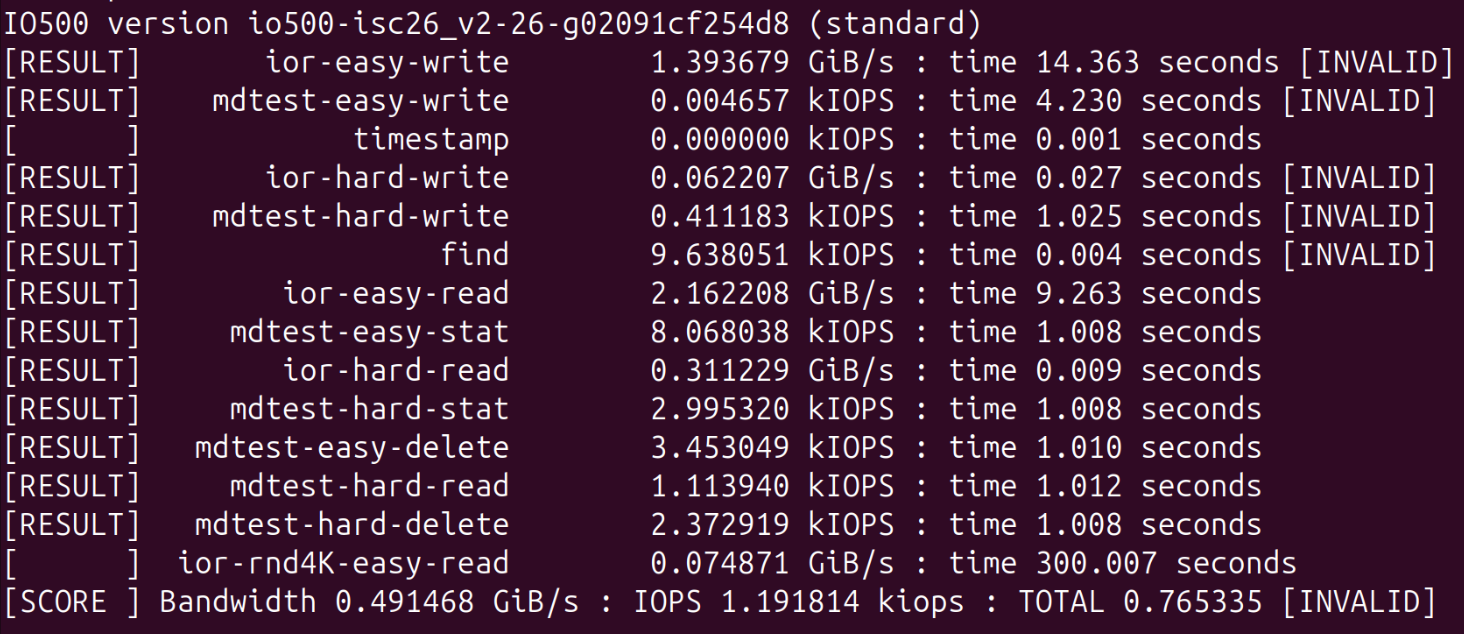
\includegraphics[width=0.90\textwidth]{figures/io500_invalid_run.png}
%\caption{Example of an invalid IO500 run using a shortened benchmark.
%The test was used to verify the benchmark configuration and
%estimate its execution time.}
%\label{fig:io500-invalid-run}
%\end{figure}


\del{These short runs were useful for testing the experimental setup. They
are also used later in this work as a cheaper way to evaluate many
configurations.}
\note{All this part above needs to be in methodology not background.}

\subsubsection{Configuration and tuning}

The performance obtained by IO500 depends not only on the storage
hardware, but also on how the benchmark uses the available resources.
Several parameters can therefore be changed between two executions. At the compute level, the configuration can include the number of
compute nodes and the number of processes used by the benchmark. The
placement of processes can also affect the communication between the
compute nodes and the storage system.

The file system configuration provides additional parameters. For
example, the number of storage targets used by a file and the way data
is distributed across these targets can affect I/O performance. Other
parameters, such as transfer size and block size, can also influence
the measured performance.

These parameters are not independent. A configuration that performs
well with a small number of processes may not provide the same
performance when more processes or nodes are used. \del{Similarly, changing
a file-system parameter can have a different effect depending on the
number of clients accessing the storage system.} The result is a multi-dimensional configuration space in which each
combination of parameter values corresponds to a possible IO500
execution. 

\del{In this internship, this configuration space is explored
using IOPS and different search strategies.}

\del{The exhaustive search described later in this report evaluates the
configurations in the selected parameter space and provides a reference
for the other search strategies. Bayesian Optimization and random
search can then be evaluated according to how quickly they find
high-scoring configurations.}

\note{The text above is objective and methodology.}

\subsection{IOPS}

The previous section showed that tuning IO500 can require a large number of
benchmark evaluations. Each evaluation can take a significant amount of
cluster time, making manual testing and exhaustive search difficult in
practice. To automate this process, \replace{the internship uses}{we use} IOPS~\cite{iops}. IOPS is a
framework developed within the TADaaM team to run parameter studies on
HPC systems. It can generate benchmark runs, submit them to the cluster,
collect their results, and use these results to guide a search.

This makes IOPS suitable for the IO500 tuning problem. Instead of manually
changing the parameters and launching each benchmark, the parameters and
their possible values can be described in an IOPS configuration file. The
search strategy can then select which configuration should be evaluated
next.

In this \replace{internship}{work}, IOPS is used as the common framework for comparing
different search strategies. This allows exhaustive search, random search,
and Bayesian Optimization to use the same benchmark and experimental
environment. The main difference between the experiments is therefore the
way in which the next configuration is selected.


\del{IOPS also stores the results of the experiments. This is particularly
useful for this study because IO500 evaluations are expensive. Once a
configuration has been evaluated, its result can be reused without running
the benchmark again. This feature is later used to perform part of the
comparison offline.}


\subsubsection{IOPS workflow}

An IOPS experiment starts with a configuration file that describes the
parameters to be tested and the benchmark to be executed. From this
configuration, IOPS generates the different parameter combinations that
will be evaluated.

For each evaluation, IOPS prepares the benchmark command with the selected
parameters and submits the job to the HPC cluster. The cluster scheduler
then executes the benchmark on the allocated resources. Once the execution
is finished, IOPS collects the output and extracts the performance result. The result is associated with the parameters used for the corresponding
run. It can then be used by the search strategy to select the next
configuration to evaluate. The process is repeated until the search budget
is reached or all configurations have been evaluated.

IOPS also provides a cache for the results. When a configuration has
already been evaluated, its result can be retrieved from the cache instead
of running the benchmark again. This is particularly useful for IO500,
where a single valid evaluation can require a significant amount of
cluster time. The general workflow used in this internship is summarised
in Figure~\ref{fig:iops-workflow}.

\begin{figure}[H]
    \centering
    \begin{tikzpicture}[
        font=\small,
        stage/.style={
            draw=wfstroke, fill=wffill, line width=0.7pt,
            rounded corners=3pt, align=center,
            text width=25mm, minimum height=11mm, inner sep=1.8mm
        },
        store/.style={
            draw=wfcachestroke, fill=wfcachefill, line width=0.7pt,
            cylinder, shape border rotate=90, aspect=0.30,
            align=center, text width=21mm, minimum height=12mm,
            inner sep=1.6mm
        },
        flow/.style={
            -{Stealth[length=2.4mm, width=1.9mm]},
            line width=0.7pt, draw=wfstroke
        },
        reuse/.style={
            flow, draw=wfcachestroke,
            dash pattern=on 2.2pt off 1.8pt
        },
        lbl/.style={
            font=\scriptsize\itshape, text=wfstroke,
            inner sep=2pt, fill=white
        }
    ]

    \node[stage] (cfg)    at (0,    2.1)  {Configuration\\file (YAML)};
    \node[stage] (search) at (0,    0)    {Search\\strategy};
    \node[stage] (submit) at (5.5,  0)    {Job submission\\(scheduler)};
    \node[stage] (run)    at (11.0, 0)    {IO500\\execution};
    \node[stage] (result) at (11.0, -4.2) {Result\\extraction};
    \node[store] (cache)  at (0,    -4.2) {Result\\cache};

    \draw[flow]  (cfg)    -- (search);
    \draw[flow]  (search) -- node[lbl, above] {next configuration} (submit);
    \draw[flow]  (submit) -- (run);
    \draw[flow]  (run)    -- (result);
    \draw[flow]  (result) -- node[lbl, above] {store result} (cache);
    \draw[reuse] (cache)  -- node[lbl, right=1.5mm, align=left]
                              {reuse cached\\results} (search);

    \end{tikzpicture}
    \caption{Workflow of an IO500 experiment in IOPS. The search strategy
    selects the next configuration, IOPS submits the corresponding
    benchmark job to the cluster scheduler, and the extracted result is
    stored in the cache. Configurations that have already been evaluated
    are served from the cache instead of being run again.}
    \label{fig:iops-workflow}
\end{figure}

This workflow allows the benchmark execution and the search strategy to
remain separate. The same IO500 experiment can therefore be used with
different search strategies without changing the rest of the experimental
setup.


\subsubsection{Parameter configuration}

IOPS uses a YAML configuration file to describe an experiment. The file
contains the parameters to explore, the values that can be used for each
parameter, and the commands needed to run the benchmark. This makes the
experimental setup explicit and allows the same study to be reproduced
later.

For the IO500 experiments, the configuration file describes the parameters
that can affect the benchmark performance. For example, the number of
compute nodes, the number of processes per node, and storage-related
parameters can be included in the study. Each possible value is specified
in the YAML file, and IOPS uses these values to generate the configurations
to evaluate.

A simplified example of the configuration used for this work is shown
below:

\begin{minted}[
    fontsize=\small,
    frame=lines,
    breaklines=true
]{yaml}
benchmark:
  name: io500

parameters:
  nodes:
    values: [1, 2, 4]
  processes_per_node:
    values: [1, 2, 4, 8]
\end{minted}

\del{For each combination of parameter values, IOPS creates an experiment and
runs IO500 with the corresponding configuration. The resulting IO500
score is then associated with the parameter combination.}

The YAML configuration defines the benchmark and the parameter space to
explore, while the search strategy determines how configurations are
selected. Therefore, the same parameter space can be explored using
different strategies available in IOPS, such as exhaustive search, random
search, or Bayesian Optimization.

During the internship, an example IO500 YAML configuration was also
created as part of the work. This configuration provides a reproducible
description of the experiment and can be reused to run IO500 through
IOPS.


\subsubsection{Search strategies}

IOPS supports several search strategies for exploring a parameter space.
The search strategy determines which configuration is selected at each
step of an experiment. The simplest approach is exhaustive search. It evaluates all possible
parameter combinations and provides the best result within the defined
search space. However, the number of configurations can quickly become
too large. \del{In this internship, exhaustive search was first used as a
reference for the other strategies.}

Random search selects configurations randomly from the parameter space.
It does not use the results of previous evaluations to select the next
configuration. It is therefore simple to use and provides a useful
baseline for comparison. \add{Moreover, IOPS can associate a budget with
random search, expressed as a number of tests or a number of core hours.
This makes the strategy suitable when the objective is to explore a large
parameter space without relying on a guided method.}

Bayesian Optimization (BO) is the main search strategy investigated in
this \replace{internship}{work}. It uses the results of previous evaluations to guide the
selection of new configurations. However, BO is not a single fixed
method. Its behaviour depends on several choices, such as the surrogate
model, the acquisition function, the exploration parameters, the number
of initial evaluations, and the total search budget.

These parameters can have a significant effect on the quality of the
search. For example, the surrogate model determines how the results of
previous evaluations are represented, while the acquisition function
controls how new configurations are selected. The exploration parameters
also influence the balance between testing promising configurations and
exploring less tested areas of the parameter space.

\del{In this internship, different BO configurations were therefore evaluated
rather than treating Bayesian Optimization as a single method. The
objective was to determine which combination of parameters performs best
for the IO500 tuning problem under a limited number of evaluations.}
\note{This belongs to methodology}

The search component of IOPS was also extended during the internship with
additional optimization methods. The Tree-structured Parzen Estimator
(TPE) was implemented as an additional search strategy. Iterated Racing
(irace) and Covariance Matrix Adaptation Evolution Strategy (CMA-ES) were
also considered as possible extensions. All these strategies can use the same IOPS experiment and parameter
space. 

\subsubsection{Result management and caching}

IOPS stores the result of each experiment together with the parameters
used for that experiment. This allows the results to be kept and reused
after the benchmark execution.  \del{This feature is particularly useful for this internship because IO500
evaluations are expensive. Once a configuration has been evaluated, it
does not need to be run again if its result is already available.} The results \del{used in this work} are stored in an SQLite database. Each
entry associates a parameter configuration with its corresponding
benchmark result. The database therefore provides a persistent record of
the experiments performed during the study.

The cache also makes it possible to replay an experiment without using
the cluster. For example, IOPS can use the previously stored results in
cache-only mode instead of submitting new benchmark jobs. This was used
to compare search strategies offline using the same set of IO500
measurements.

\del{This separation between benchmark execution and result analysis is
important for the experimental study. Expensive measurements only need to
be performed once, while different search strategies can be evaluated
later using the stored results.}


\subsection{Bayesian Optimization}

\replace{Bayesian Optimization (BO)}{BO} is a search method designed for
problems where evaluating \add{all possible} configurations is \add{too}
expensive. This makes it suitable for the IO500 tuning problem, since each
configuration requires running the benchmark on an HPC system and can
therefore consume a significant amount of cluster time. \add{In addition,
the number of parameter combinations is very large.} The main idea of BO
is to use the results of previous evaluations to decide which
configuration should be evaluated next. \add{In other words, it explores
the parameter space selectively rather than uniformly.}

Let the configuration of a benchmark be represented by a vector of
parameters $x$, and let $f(x)$ be the performance obtained by running
IO500 with this configuration. The objective is to find a configuration
that maximises $f(x)$. In a large search space, evaluating every possible
configuration may be too expensive. BO instead tries to find a good
configuration with a limited number of evaluations.

BO starts with a small number of initial configurations. These
configurations are evaluated using the real objective function, in our
case the IO500 benchmark. The obtained results form the initial set of
observations. BO then builds a model, called a \emph{surrogate model},
from these observations. This model provides an approximation of the
relationship between the configuration parameters and the expected
performance. The surrogate model is used because evaluating the real objective
function is expensive, while evaluating the model is much cheaper. The
model can therefore be used to estimate which parts of the search space
are promising before running another IO500 experiment.

After building the surrogate model, BO uses an \emph{acquisition function}
to select the next configuration to evaluate. The acquisition function
uses the information provided by the model to decide where the next
evaluation should be performed. It can favour configurations that are
expected to provide a high score, but it can also favour configurations
where the model is uncertain.

This creates a balance between \emph{exploitation} and \emph{exploration}.
Exploitation means testing configurations that are expected to perform
well according to the current model. Exploration means testing less
certain configurations in order to obtain new information about the
search space. Finding a good balance between these two behaviours is
important because focusing only on exploitation can cause the search to
remain in a local region, while excessive exploration can waste
evaluations on configurations that are unlikely to perform well.

The process is then repeated. The selected configuration is evaluated with
IO500, its measured score is added to the observations, and the surrogate
model is updated. A new configuration is then selected using the updated
model. In this way, each expensive evaluation provides information that
can be used to improve the following choices.

The general workflow of \replace{Bayesian Optimization}{BO} is illustrated in
Figure~\ref{fig:bo-workflow}.

\begin{figure}[ht]
    \centering
    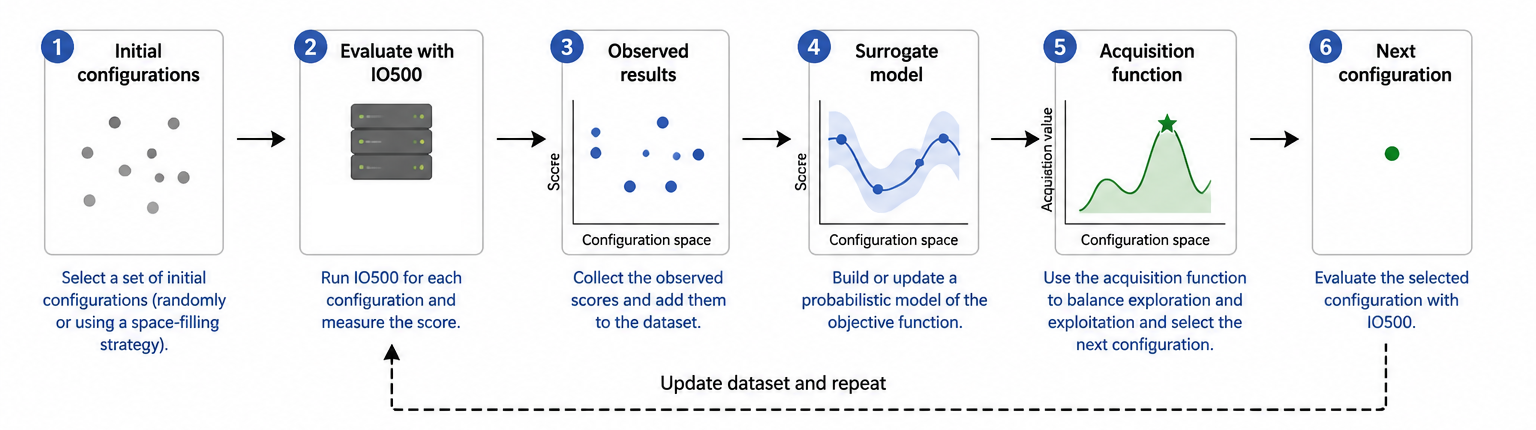
\includegraphics[width=\textwidth]{figures/boworkflow.png}
    \caption{General workflow of Bayesian Optimization for IO500 tuning.}
    \label{fig:bo-workflow}
\end{figure}

An important point is that \replace{Bayesian Optimization}{BO} is not a single fixed
algorithm. Different surrogate models and acquisition functions can be
used, and their parameters can change the behaviour of the search. In
this work, we consider Gaussian Processes (GP), Random Forests (RF), and
Extra-Trees (ET) as surrogate models. We also consider Expected
Improvement (EI), Probability of Improvement (PI), and Lower Confidence
Bound (LCB) as acquisition functions.

Other parameters also affect the search, such as the number of initial
evaluations and the parameters controlling exploration. The total number
of evaluations, or search budget, is another important factor because it
determines how many \del{expensive IO500} runs can be performed.

For \replace{this reason}{these reasons}, the objective of the study is
not simply to determine whether \replace{Bayesian Optimization works}{BO
works in this context}\add{, but also to identify which combination of BO
choices is most effective for the IO500 tuning problem}. \del{We also want
to determine which combination of BO choices is the most effective for the
IO500 tuning problem.} The different \add{BO} configurations are evaluated
under the same experimental conditions and with a limited number of
evaluations. Their performance can then be compared with the exhaustive
and random search strategies described previously.
